\section{Summary diagram}

\begin{figure}[!htb]
    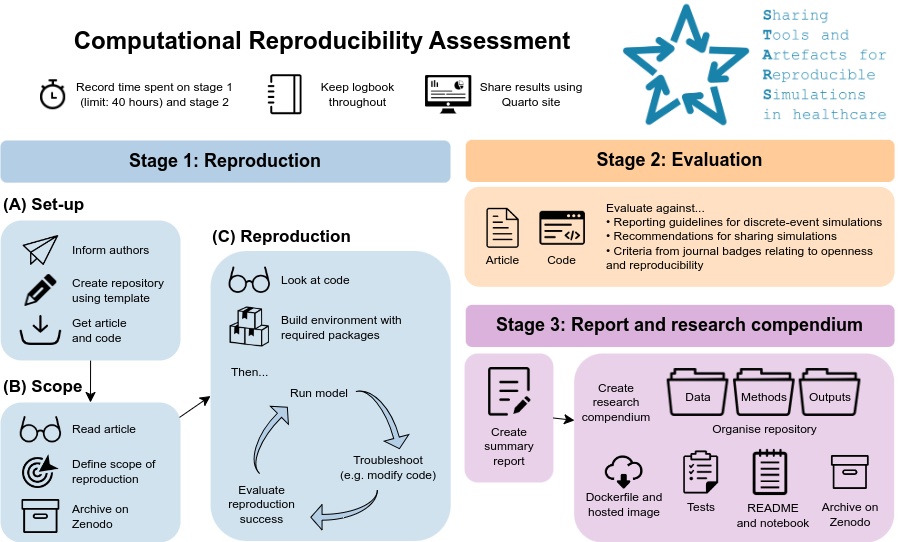
\includegraphics[width=1\linewidth]{images/stars_wp1_workflow_4.drawio.png}
    \caption{Workflow for assessing the computational reproducibility of discrete-event simulation models on STARS.}
\end{figure}

\newpage
\section{Introduction}

In this protocol, we are focused on the \textbf{computational reproducibility} of simulation models. This is defined as the ability to get consistent results with a prior study when using  the same data and methods as that study. We are focusing on models developed using \textbf{Python and R}, as these are popular free and open-source software (FOSS) for the development of models like discrete-event simulation (DES).\autocite{monks_computer_2023}

This protocol will be used to assess the computational reproducibility of \textbf{six DES models}. These are selected from the models identified by \textbf{Monks and Harper 2023}.\autocite{monks_computer_2023} The selection criteria are that: (i) the model code is publicly available, (ii) the model is created using Python or R, and (iii) the code has an open license (either already published, or added upon request from the STARS team).

Throughout the study, results will be openly available and shared via a \textbf{Quarto website}. This will compile information on the reproduction of the article. This includes the notebooks (.ipynb or .Rmd) producing the items in the scope, as well as a chronological log of work using Quarto blog posts, and then later, the reproduction report and detailed study results.

The protocol will often refer to our \textbf{template repository} which can be viewed here -\url{https://github.com/pythonhealthdatascience/stars_reproduction_template}. As you will see, one of the first steps for researchers will be to use this template to set-up their repository for the reproducibility assessment. \hl{Change to link to Zenodo before publishing}

There are \textbf{three key stages} to this protocol which you should \textbf{work through in the following order}:
\begin{enumerate}
    \item Assessment of computational reproducibility
    \item Evaluation against guidelines
    \item Summary report and research compendium
\end{enumerate}

However, we first introduce two important processes that will need to be \textbf{completed during some or all of the stages}:
\begin{itemize}
    \item Keeping a detailed record of work using a \textbf{logbook}
    \item \textbf{Timing} how long tasks take to complete
\end{itemize}

\newpage
\section{Logbook}

Throughout \textbf{all of the stages} below, you should keep a \textbf{logbook}.

This is a detailed record of work recorded using \textbf{Quarto blog posts}, using the template provided. As suggested by Ayllón et al. 2021\autocite{ayllon_keeping_2021} in their guidelines for keeping modelling notebooks, these posts will be \textbf{daily}, dated, chronological entries. \textbf{Tags} will be used to help indicate the activity on each day, and enable posts to be filtered by activity. Keeping a detailed log will support later understanding of what was done, and support preparing of final documents like the summary report.

Each entry in the logbook should contain the:
\begin{itemize}
    \item \textbf{Researcher name} and \textbf{date}
    \item \textbf{Tags} (e.g. setup, scope, read, reproduce, guidelines, compendium, report)
    \item \textbf{Time} spent on tasks (if applicable)
    \item \textbf{Comprehensive} record of work. This should include record of working through each stage in the protocol, detailing \textbf{successes} and any \textbf{issues} faced, any \textbf{solutions} found to problems, and any \textbf{changes made to the model code} (noting where and how the code was changed). It may be relevant to include links to particular versions of a file or repository such as via the Git commit history.
    \item Clear statement if and when each item in the scope is considered to have been \textbf{successfully reproduced}.
\end{itemize}

\newpage
\section{Timing}

During the first and second stages of your study (\textbf{assessment of computational reproducibility}, and \textbf{evaluation against guidelines}) you should \textbf{time how long each task takes}. Whilst timing, it is important you timestamp:
\begin{itemize}
    \item When you finish reproducing each item within the scope
    \item When you have finished working on evaluation of artefacts (badges and recommendations on sharing), and when you have finished working on evaluation of the article (STRESS-DES and ISPOR-SDM)
\end{itemize}

These times should be recorded within the logbook alongside each activity (e.g. 12:10 to 12:45). The times should be monitored with a \textbf{maximum of fourty hours} allowed for the first stage (attempting to reproduce the study), as in Krafczyk et al. 2021.\autocite{krafczyk_learning_2021} This cut-off is implemented as we anticipate there would be little more to learn from spending longer than that time on reproducing a single study.

The only exceptions to this timing are:
\begin{itemize}
    \item \textbf{Computation time}. This is at the researcher's discretion. For example, you should include short run times where you are still continuously working on the study. You should exclude longer run times where you are no longer working towards the assessment of computational reproducibility - for example, if you set the simulation to run for five minutes whilst going to make a cup of tea.
    \item \textbf{Time spent by other researchers}. You should record the time spent by the primary researcher on completing tasks, and time spent in discussion with other researchers. However, if other researchers spend time preparing for those discussions (e.g. reading the article, looking over the work), this does not need to be recorded.
\end{itemize}